%\documentclass[preprint,12pt]{elsarticle}
\documentclass[11pt]{article}
\usepackage[ansinew]{inputenc}
\usepackage{epsfig}
\usepackage{amsfonts}
\usepackage{amssymb}
\usepackage{subfigure}
\usepackage[usenames]{color}
\usepackage{comment}
\usepackage{graphicx}
\usepackage{verbatim}
\usepackage{geometry}
\usepackage{setspace}
\usepackage{epsfig}
\usepackage{subfigure}
\usepackage[usenames]{color}
\usepackage{soul}
\usepackage{comment}
\usepackage{multirow}
\usepackage[cmex10]{amsmath}
\usepackage{bm}
\usepackage{setspace}

\usepackage{algorithm}
\usepackage{algpseudocode}
\usepackage{psfrag}


%--------------------------------------------------
\newcommand{\comm}[1]{{\it \color{red} \st{#1}}}
% \newcommand{\comm}[1]{}

\newcommand{\Borcomm}[1]{{\it \color{OliveGreen} [#1]}}

\newcommand{\vectornorm}[1]{\left|\left|#1\right|\right|}

\begin{document}

\title{Channel Selection in WLANs using Channel Bonding}  
%\date{}

%\author{Boris Bellalta\\Universitat Pompeu Fabra, Barcelona}

\maketitle

%\begin{abstract}
%x
%\end{abstract}



% ----------------------------------------------------
% ----------------------------------------------------
% ----------------------------------------------------
% ----------------------------------------------------

\section{Introduction} \label{Sec:Intro}

In Figure \ref{Fig:RandomScenario} a random scenario with several overlapping WLANs is shown (each circle represents the coverage area of a WLAN). They will interfere each other if they use the same channels. Therefore a solution is to select a different channel for each BSS. However, as each BSS can use several basic channels to increase its performance, to assign orthogonal group of channels to overlapping BSS may be more difficult. Then, each BSS have to decide how many channels it will use, and what are those channels to maximize its performance.

\begin{figure}[t!]
	\centering
	
\epsfig{file=RandomScenario.eps,scale=0.5}
	\caption{Overlapping BSSs: A random scenario}\label{Fig:RandomScenario}
\end{figure}

In Figure \ref{Fig:Ex_ChannelBonding} we have $3$ WLAN Basic Service Sets (BSSs). The first BSS overlaps with the second BSS, and the second BSS overlaps with the third one. In the a) case, all of them use $4$ basic channels. However, as they share at least one of the basic channels, they have to agree on a temporal schedule to transmit. In the b) case, each BSSs uses only $2$ channels, though they are not the same with the others overlapping BSSs. Therefore, they can transmit during all the time.

\begin{figure}[t!]
	\psfrag{bss1}[][][0.6]{BSS $1$}
	\psfrag{bss2}[][][0.6]{BSS $2$}
	\psfrag{bss3}[][][0.6]{BSS $3$}		
	\psfrag{time}[][][1]{t}	
	\psfrag{a}[][][1]{a)}		
	\psfrag{b}[][][1]{b)}			
	\centering
	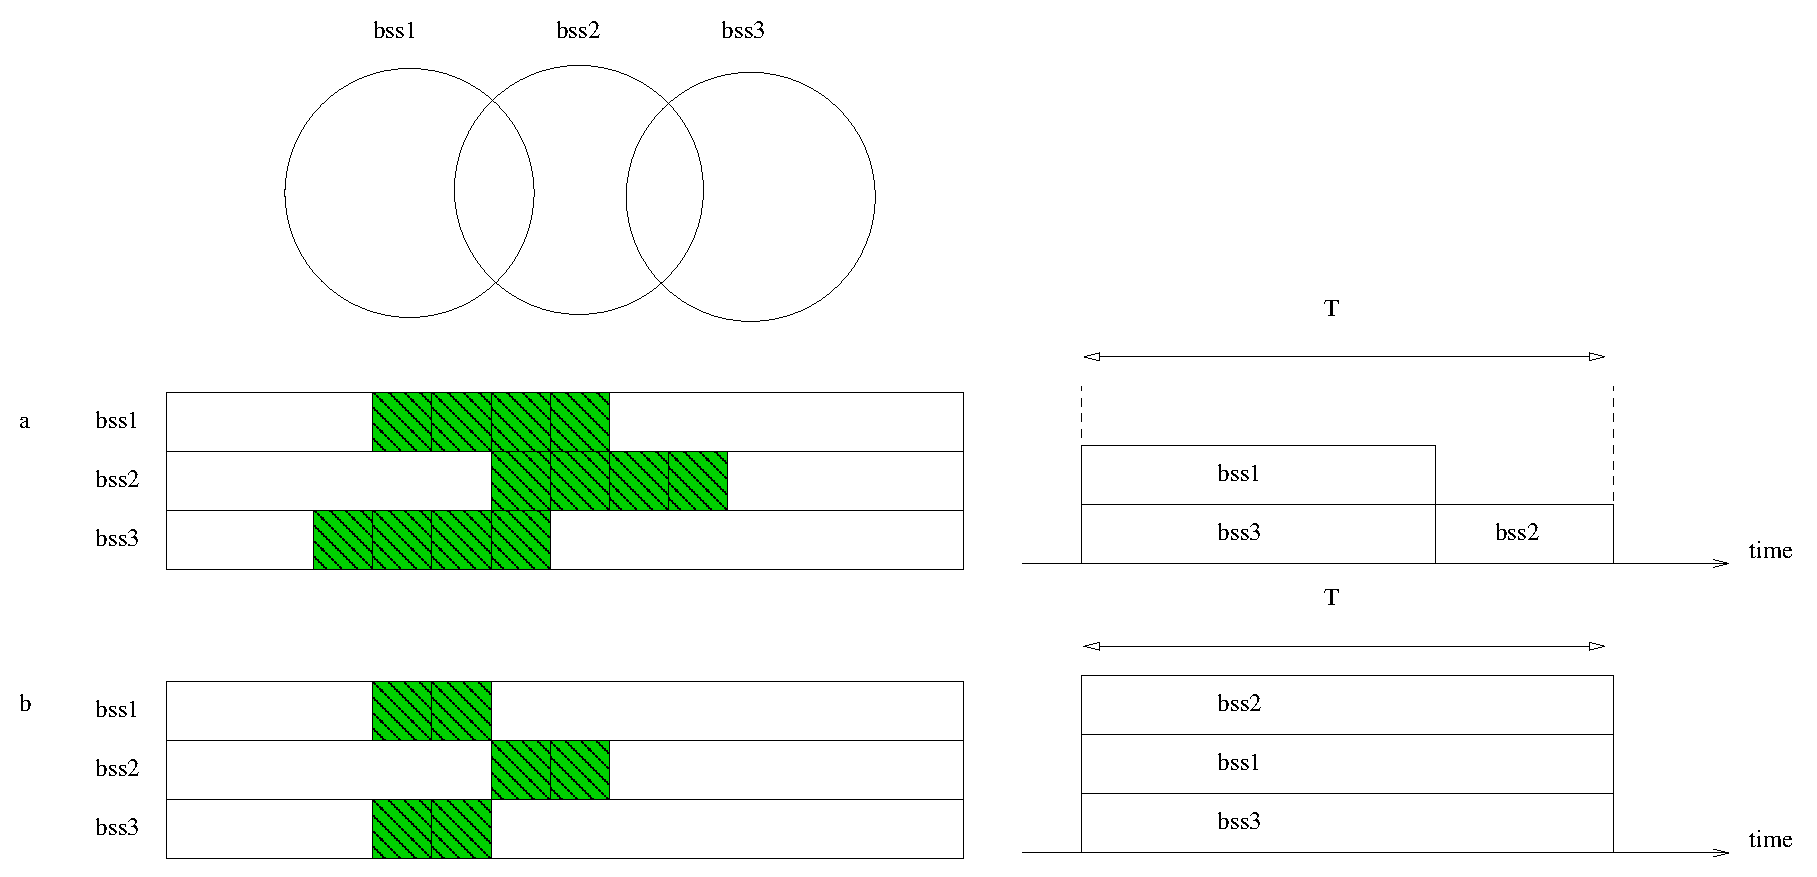
\epsfig{file=Ex_ChannelBonding.eps,scale=0.5}
	\caption{Example}\label{Fig:Ex_ChannelBonding}
\end{figure}


Some assumptions:

\begin{enumerate}
	\item Should we play with the power control too? We can assume that the transmission power is fixed.
	\item All the BSS have the same capabilities (i.e. can use the same number of channels).
	\item The throughput of an isolated BSS using $n$ basic channels is $S(n)$. 
	\item A BSS overlaps with another BSS if at least one of its $n$ used channels is shared by another BSS in the same geographical area.
	\item The throughput of a BSS when it has $|\mathcal{K}|$ overlapping BSSs is $$S'_i(n_i)=S_i(n_i)-\sum_{\forall j \in \mathcal{K}}{S'_j(n_j)}$$
	\item It can be assumed that all the BSSs that overlap can agree on a temporal schedule to transmit without colliding. For example, two BSS overlapping can agree that each one will transmit alternatively every $50$ msecs. In case that there are thee BSS, see Figure \ref{Fig:Ex_ChannelBonding}.
\end{enumerate}

Goals:

\begin{enumerate}
	\item The throughput of the $i$th BSS is the $S'_i(n_i)=\frac{T_i}{T}S_i(n_i)$.
	\item Find $n_i$, its location, and $T_i$ to maximize its performance / the performance of all the BSSs that overlap. Does proportional Fairness apply here?
\end{enumerate}

\clearpage

\section{Toy Scenarios}

In Figures \ref{Fig:Fig_Case1}, \ref{Fig:Fig_Case2} and \ref{Fig:Fig_Case3}, we have some detailed scenarios.

\begin{figure}[t!]
	\psfrag{bss1}[][][1]{BSS 1}
	\psfrag{bss2}[][][1]{BSS 2}	
	\psfrag{ap}[][][0.6]{AP}
	\psfrag{sta}[][][0.6]{STA}
	\psfrag{The cloud}[][][1]{The Cloud}	
	\centering
	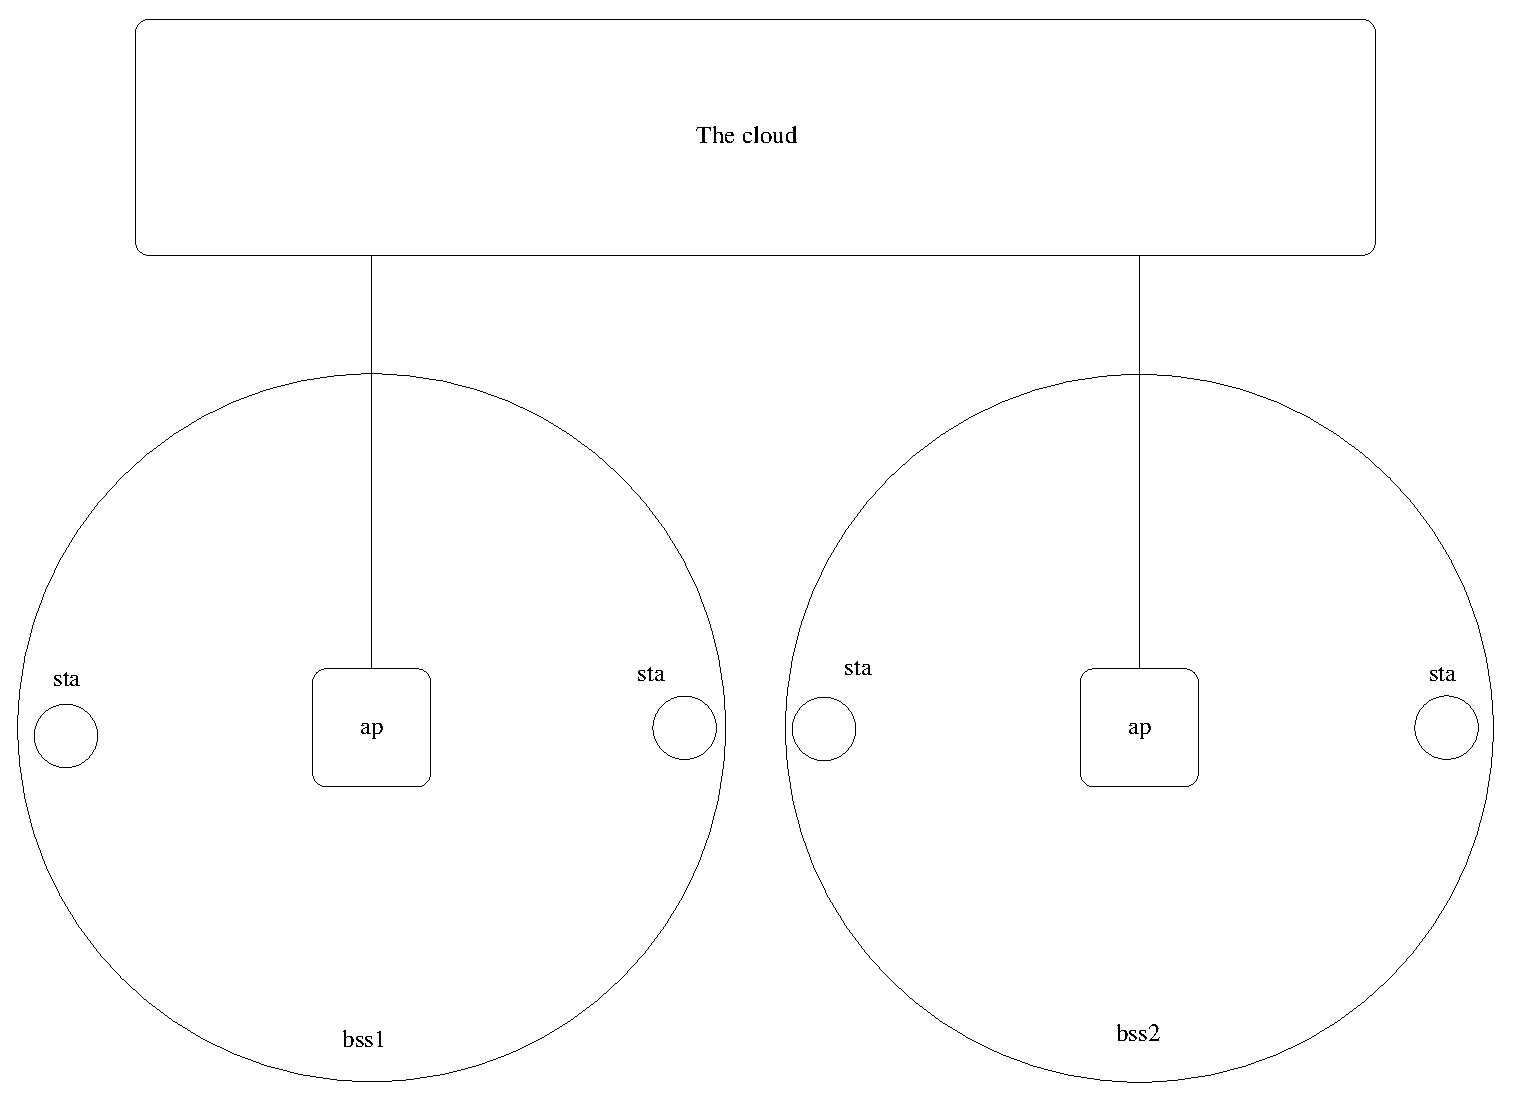
\epsfig{file=Fig_Case1.eps,scale=0.5}
	\caption{Non-overlapping BSS}\label{Fig:Fig_Case1}
\end{figure}

\begin{figure}[t!]
	\psfrag{bss1}[][][1]{BSS 1}
	\psfrag{bss2}[][][1]{BSS 2}	
	\psfrag{ap}[][][0.6]{AP}
	\psfrag{sta}[][][0.6]{STA}
	\psfrag{The cloud}[][][1]{The Cloud}	

	\centering
	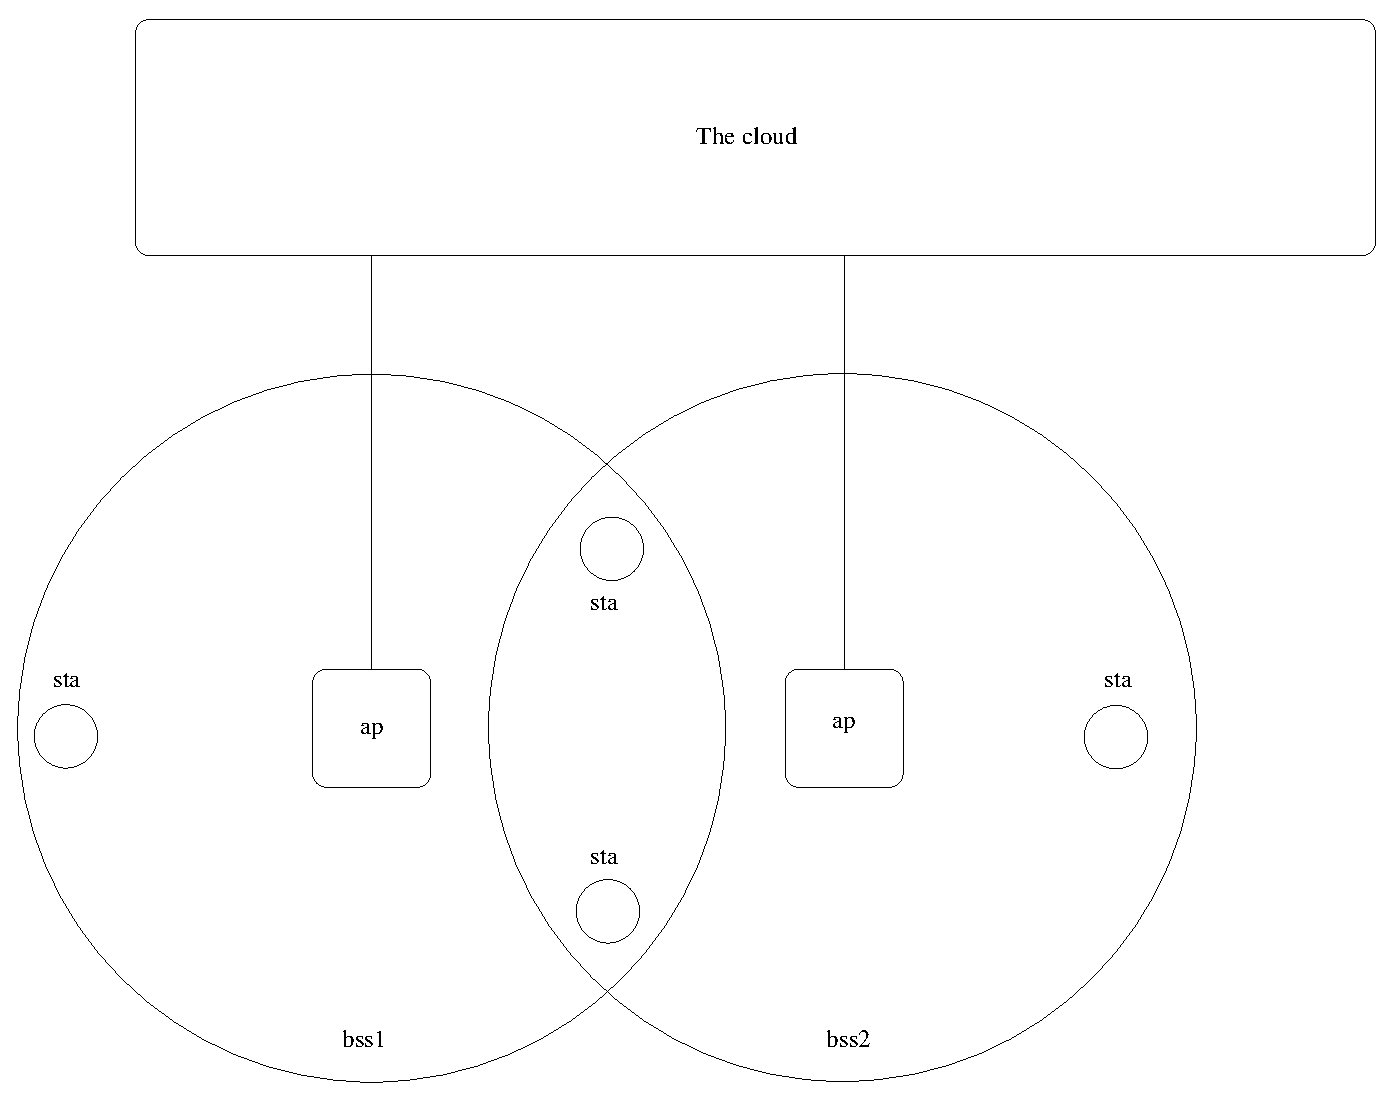
\epsfig{file=Fig_Case2.eps,scale=0.5}
	\caption{Overlapping BSS. APs can not communicate.}\label{Fig:Fig_Case2}
\end{figure}

\begin{figure}[t!]
	\psfrag{bss1}[][][1]{BSS 1}
	\psfrag{bss2}[][][1]{BSS 2}	
	\psfrag{ap}[][][0.6]{AP}
	\psfrag{sta}[][][0.6]{STA}
	\psfrag{The cloud}[][][1]{The Cloud}	

	\centering
	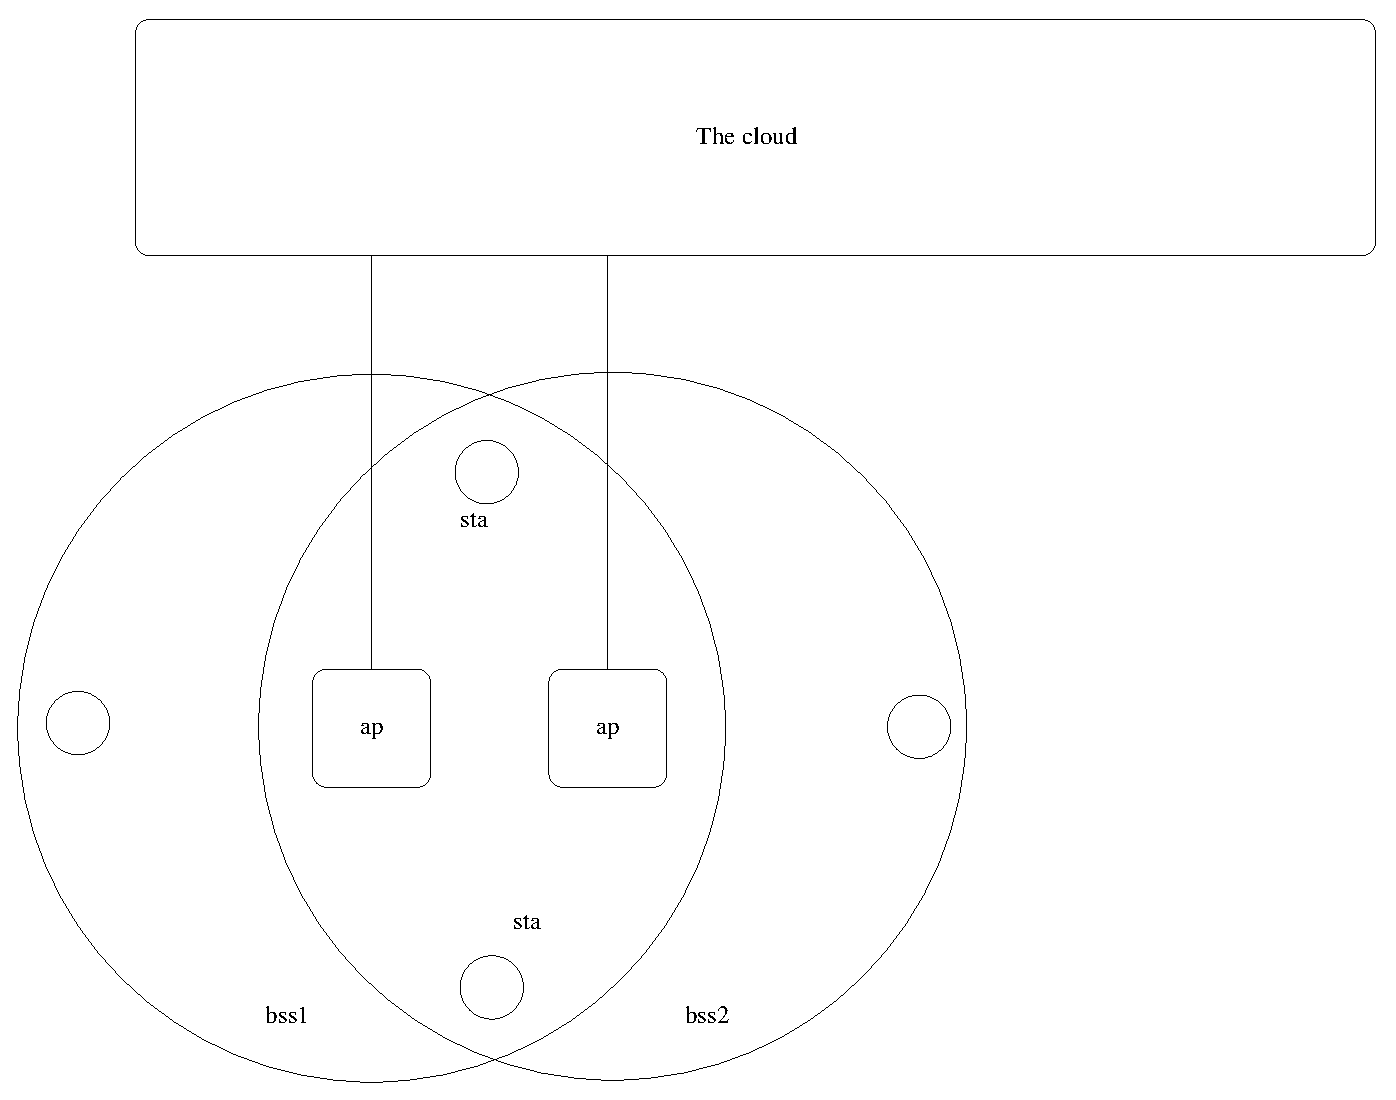
\epsfig{file=Fig_Case3.eps,scale=0.5}
	\caption{Overlapping BSS. APs can communicate}\label{Fig:Fig_Case3}
\end{figure}


\end{document}
